\documentclass[../../thesis.tex]{subfiles}

\begin{document}

% \section{Initial Experimentation and Model Development}
% \TODO{This section is under construction. Contemplating if i should even include it at all in some form.}

% The overarching objective in creating our model is to learn more expressive latent representations for better time series generation. We want to keep the reconstruction capabilities of the tokenization model at a high level, where the rationality is that if the tokenization model reconstructs well the latent representations contains all relevant information of the input. We simultaneously want enforce better class separability in the latent representations, as we hypothesize that such additional structure eases/improved learning of the generative model.\newline

% During development we encountered several problems:\newline
% When we attempted a siamese architecture, with quantization in the augmented branch, and to derive the SSL loss from the discrete representations there were a correlation problem. The codewords were very highly correlated, which resulted from the passing both views through the VQ.  $SSL(z_q,z_q')$ \newline
% In an attempt to solve this we attempted to derive the SSL loss from the continuous latent representations, but the resulting discrete latent representations performed poorly on the downstream classification task. Separability problem: $SSL(z,z')$ \newline
% The solution was to remove the VQ in the augmented branch and rather derive the SSL loss from $z_q$ and $z'$. Solution: $SSL(z_q,z')$ \newline

% Overfitting problem: Using $SG()$ on augmented branch / Not using augRecons \newline

\section{Main Experiments}
\TODO{This section i need som assistance with. Find it difficult to write anything smart.}

To evaluate our model NC-VQVAE and address the research questions, we compare it to the naive VQVAE using both Barlow Twins and VIbCReg as self-supervised learning methods. Additionally, as we are interested in the effect of augmentations on representation learning, for each SSL method we train three distinct models using different sets of augmentations. Furthermore, each configuration is trained using four different seeds, resulting in a total of 364 models trained at each stage. All experiments were run on the Idun HPC cluster \cite{Idun}, using several compute nodes. The total training time of all 728 models was approximately 700 hours. 


\subsection{Implementation details}

In our implementation, we closely follow to the methodology outlined in \cite{TimeVQVAE}, particularly in the design and deployment of the encoder, decoder, and codebook. The code base for the project is found at \url{https://github.com/erlendlokna/Generative-SSL-VQVAE-modelling}

\subsubsection{Time Frequency Modelling}
We utilize the Short Time Fourier Transform (STFT) and its inverse (ISTFT) for time-frequency modeling, using the functions \texttt{torch.stft} and \texttt{torch.istft}, respectively. Consistent with \cite{TimeVQVAE}, we set the primary parameter $\texttt{n}_{\texttt{fft}}$ to 8 and use default parameters for others. This configuration yields a frequency axis spanning $[1, 2, 3, 4, 5]$ and a time axis half the length of the original.

\subsubsection{Encoder and decoder}

The encoder and decoder architectures closely resemble those described in \cite{nadavbh12}, with further adaptations from \cite{TimeVQVAE}.\newline

\begin{figure}[h]
    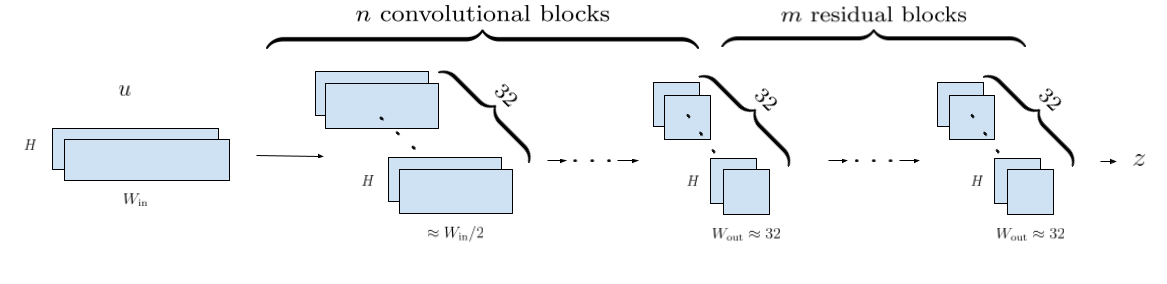
\includegraphics[scale = 0.30]{VQVAE Encoder.png}
    \centering
    \caption{Overview of the encoder architecture. The decoder architecture is simply obtained by reversing the arrows and switching out the convolutional block for transposed convolutional blocks.}
    \label{fig:VQVAE Encoder}
\end{figure}
As illustrated in Figure \ref{fig:VQVAE Encoder}, the encoder consists of $n$ downsampling convolutional blocks (\texttt{Conv2d - BatchNorm2d - LeakyReLU}), followed by $m$ residual blocks (\texttt{LeakyReLU - Conv2d - BatchNorm2d - LeakyReLU - Conv2d}). Downsampling convolutional layers are implemented with parameters: 
\[\texttt{kernel size=(3,4)}, \texttt{stride=(1,2)}, \texttt{padding=(1,1)},\] downsampling the temporal axis by a factor of 2 per block. Residual convolutional layers have parameters: 
\[\texttt{kernel size=(3,3)},\texttt{stride=(1,1)}, \texttt{padding=(1,1)}.\]
The decoder mirrors this architecture, featuring $m$ residual and $n$ upsampling layers using transposed convolutional blocks with identical parameters.\newline

The downsampling rate is determined by $2^n$, ensuring the resulting latent representation ($z$) has a width of 32. While we set the number of residual blocks $m = 4$. For an in depth walkthrough of the TimeVQVAE implementation details, we direct readers to Appendix C.3 of \cite{TimeVQVAE}.


\subsubsection{VQ}

We adopt a codebook size of 32 and a dimension of 64, utilizing exponential moving average with a decay of 0.9 and a commitment loss weight $\beta = 1$.

\subsubsection{SSL}
For both Barlow Twins and VIbCReg, we implement the projector following the guidelines in \cite{lee2024computer}. 
We use identical projectors for both methods, consisting of 3 linear layers. The first two are normalized using \texttt{BatchNorm1d}. Both hidden and output layer has dimension size set to 4096.\newline

For Barlow Twins the weight of the redundancy reduction term, $\lambda$, is set to $0.005$. The weight of the Barlow Twins loss in the NC-VQVAE is set to $\eta = 1/D$ where $D$ is the projector output dimension.\newline

For VIbCReg, the weights of the similarity loss, $\lambda$, and variance loss, $\mu$, are both set to 25, while for the covariance loss, $\nu$ is set to 100. The weight of the VIbCReg loss in the NC-VQVAE is set to $\eta = 0.01$.

\subsubsection{Augmentations}
For the reconstruction loss on the augmented brach we set the weight $\zeta$ to $0.1$. \newline 

In our experiments we consider three sets of augmentations with different characteristics. They are
\begin{itemize}
    \item Amplitude Resizing + Window Warp
    \item Slice and Shuffle
    \item Gaussian noise
\end{itemize}

\textbf{Amplitude Resizing + Window Warp} transforms in both x and y direction. The window warp augmentation randomly selects a section of the time series and speeds it up or down, and the factor is choose randomly from the interval $[0.9, 2.0]$. We interpolate in order to obtain a time series of equal length as the original. It has similar qualities to phase shift, but not uniformly and keeps endpoints fixed. The amplitude resize multiplies the time series by a factor of $1+N(0,0.2)$. This set was considered as the observed conditional distribution in some datasets, such as ShapesAll \ref{fig:datasets}, had similar overall shape, but peaked with different amplitude and at different locations. Thus the augmented view had similar characteristics as the conditional distribution of the original view as seen in Figure \ref{fig:ShapesAll_winwarp}. In many cases we will refer to this set of augmentations simply as warp. \newline

\begin{figure}[h]
    \centering
    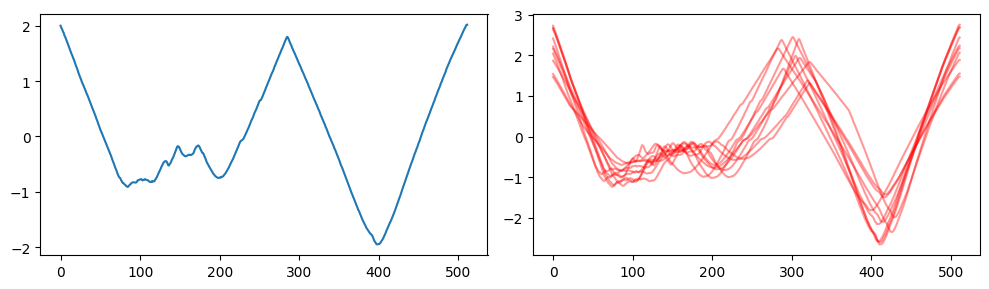
\includegraphics[scale = 0.3]{ShapesAll_winwarp.png}
    \caption{ShapesAll: Original (left), augmented (right). 15 instances of Amplitude Resizing + Window Warp applied to the original sample.}
    \label{fig:ShapesAll_winwarp}
\end{figure}

\textbf{Slice and Shuffle} crops the time series into four randomly selected sections and permutes them. For datasets with sharp modularity and few peaks, such as ElectricDevices \ref{fig:datasets}, the augmentation provides a view with peaks occurring at timestamps not seen in the training data, which is illustrated in Figure \ref{fig:ElectricDevices_SliceAndShuffel}. This could improve the reconstruction on unseen data, as well as encouraging the model to focus more on the existence of a peak rather than its specific location. For some datasets such as FordA \ref{fig:datasets}, the semantics of the dataset is preserved under this augmentation, despite their continuous nature. In many cases we will refer to this augmentation simply as slice.\newline
\begin{figure}[h]
    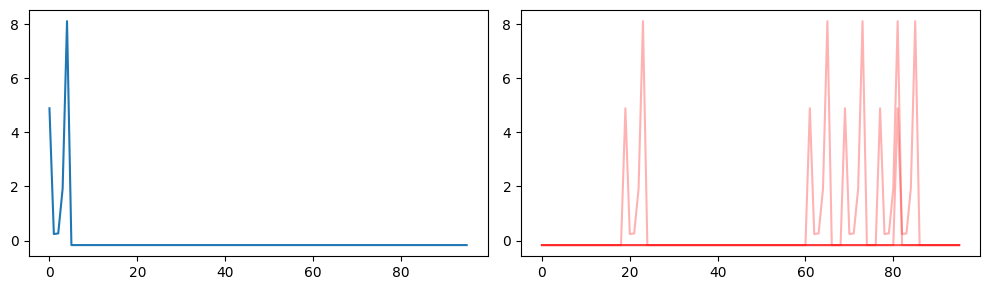
\includegraphics[scale = 0.3]{ElectricDevices_SliceAndShuffel.png}
    \centering
    \caption{ElectricDevices: Original (left), augmented (right). 5 instances of Slice and Shuffle applied to the original sample.}
    \label{fig:ElectricDevices_SliceAndShuffel}
\end{figure}

\textbf{Gaussian noise} adds a nose $\epsilon \sim N(0,0.05)$ to each datapoint in the time series. This introduces, in many cases, a substantial high frequency component as seen in Figure \ref{fig:StarLight_Gaussian}. As the naive VQVAE described in \cite{TimeVQVAE} had trouble with reconstruction of HF components, this augmentation could provide more emphasis on these. The reconstruction of the augmented views can too provide more information regarding HF components for the decoder. Of the three augmentations, gaussian noise provides the most predictable augmented views from a numerical standpoint, which might result in a SSL loss which is easier to minimize. In many cases we will refer to this augmentation simply as Gaussian or gauss.
\begin{figure}[h]
    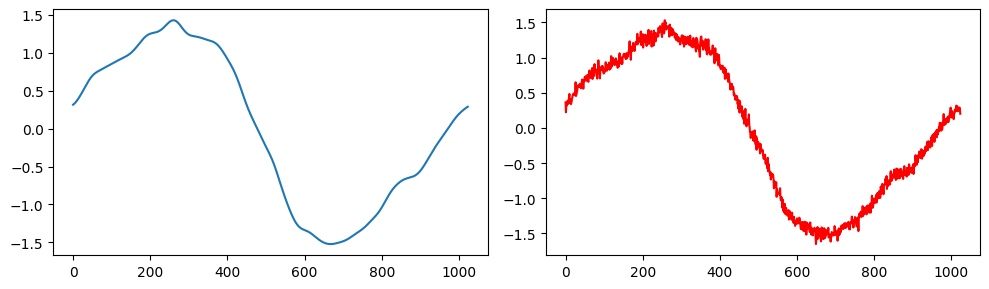
\includegraphics[scale = 0.3]{StarLight_Gaussian.png}
    \centering
    \caption{StarLightCurves: Original (left), augmented (right). One instance of Gaussian noise applied to the original sample.}
    \label{fig:StarLight_Gaussian}
\end{figure}



\subsubsection{Prior learning}
We adopt the implementation from \cite{chang2022maskgit}. In the iterative decoding algorithm, the number of iterations $T$ is set to 10, and use cosine as mask scheduling function ($\gamma$). 

\subsubsection{Training}
We utilize the AdamW optimizer with batch sizes set to 128 for stage 1 and 256 for stage 2, an initial learning rate of $10^{-3}$, cosine learning rate scheduler, and a weight decay of $10^{-5}$. Both stage 1 and stage 2 training procedures run for 1000 epochs.


\subsection{Evaluation}
For downstream classification, K-nearest neighbors (KNN) and Support Vector Machines (SVM) are implemented using scikit-learn, with $K=5$ for KNN and a linear kernel for SVM. \newline

SupervisedFCN is employed for calculating Inception Score (IS), Fréchet Inception Distance (FID), and Classification Accuracy Score (CAS). See Appendix B and C.2 of \cite{VQVAE} for detailed information.


\section{UCR Time Series Classification Archive}
The evaluation of our model NC-VQVAE is done on a subset of the UCR Time Series Archive \cite{UCRArchive2018}. The UCR archive is a collection of 128 datasets of univariate time series for classification. The different datasets in the archive span a wide range characteristics and include among others sensor, device, image-derived and simulated data. Each dataset has a predefined training and test split.\newline


\begin{table}[h]
    \centering
    \begin{tabular}{llllll}
    \toprule
    Type      & Name                    & Train & Test & Class & Length \\
    \midrule
    Device    & ElectricDevices         & 8926  & 7711 & 7     & 96     \\
    Sensor    & FordB                   & 3636  & 810  & 2     & 500    \\
    Sensor    & FordA                   & 3601  & 1320 & 2     & 500    \\
    Sensor    & Wafer                   & 1000  & 6164 & 2     & 152    \\
    Simulated & TwoPatterns             & 1000  & 4000 & 4     & 128    \\
    Sensor    & StarLightCurves         & 1000  & 8236 & 3     & 1024   \\
    Motion    & UWaveGestureLibraryAll  & 896   & 3582 & 8     & 945    \\
    ECG       & ECG5000                 & 500   & 4500 & 5     & 140    \\
    Image     & ShapesAll               & 600   & 600  & 60    & 512    \\
    Simulated & Mallat	                & 55	& 2345 & 8	   & 1024   \\
    Image     & Symbols                 & 25    & 995  & 6     & 398    \\
    Sensor    & SonyAIBORobotSurface2   & 27    & 953  & 2     & 65     \\
    Sensor    & SonyAIBORobotSurface1   & 20    & 601  & 2     & 70     \\
    \bottomrule
    \end{tabular}
    \caption{The subset of the UCR Archive considered for our experiments.}
    \label{tab:UCRsubset}
    \end{table}

The subset selected for our experiments is presented in Table \ref{tab:UCRsubset}. We choose to test on a subset, rather than on the entire UCR Archive, due to computational limitations as well as to more thoroughly investigate the effect of our models and the role of augmentations. The subset is chosen such that they span a wide range of train set sizes, lengths, classes and type, while the class distributions have visually different characteristics which can be seen from table \ref{tab:UCRsubset} and figure \ref{fig:datasets}.

\begin{figure}[h]
    \centering
    \begin{minipage}[b]{0.32\textwidth}
        \centering
        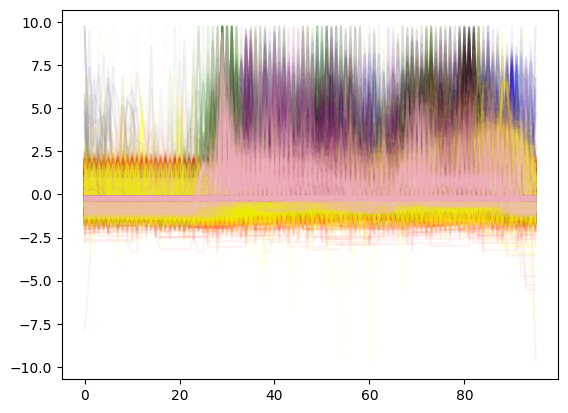
\includegraphics[width=\textwidth]{ElectricDevices}
        \caption*{ElectricDevices}
    \end{minipage}
    \hfill
    \begin{minipage}[b]{0.32\textwidth}
        \centering
        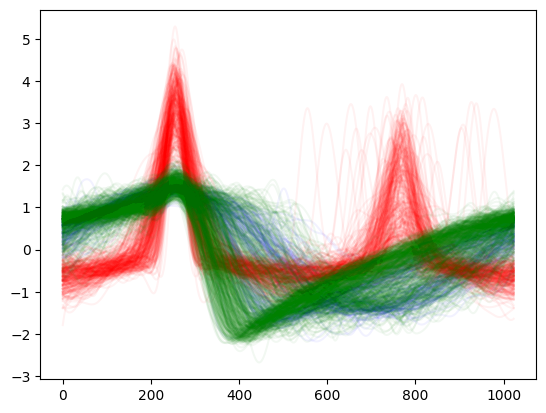
\includegraphics[width=\textwidth]{StarLightCurves}
        \caption*{StarLightCurves}
    \end{minipage}
    \hfill
    \begin{minipage}[b]{0.32\textwidth}
        \centering
        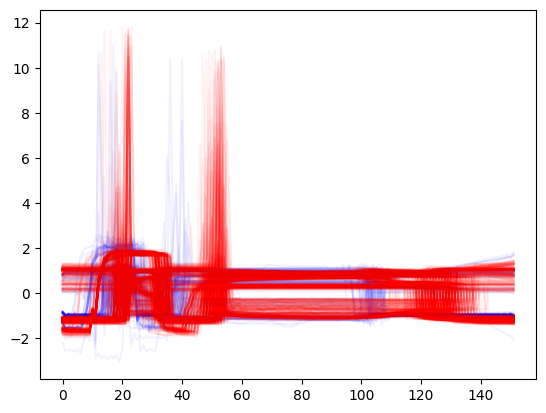
\includegraphics[width=\textwidth]{Wafer}
        \caption*{Wafer}
    \end{minipage}
    
    \vspace{0.4cm}
    
    \begin{minipage}[b]{0.32\textwidth}
        \centering
        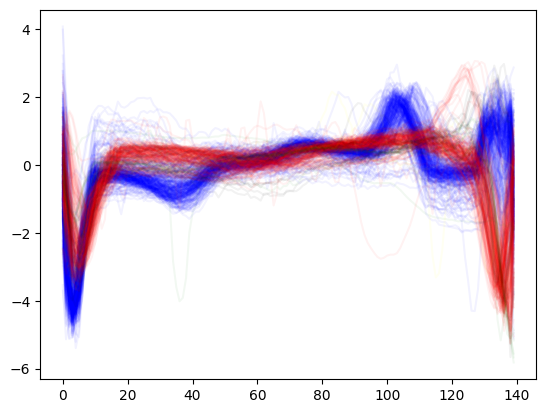
\includegraphics[width=\textwidth]{ECG5000}
        \caption*{ECG5000}
    \end{minipage}
    \hfill
    \begin{minipage}[b]{0.32\textwidth}
        \centering
        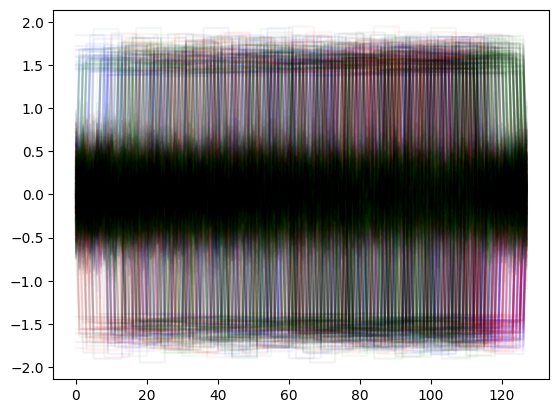
\includegraphics[width=\textwidth]{TwoPatterns}
        \caption*{TwoPatterns}
    \end{minipage}
    \hfill
    \begin{minipage}[b]{0.32\textwidth}
        \centering
        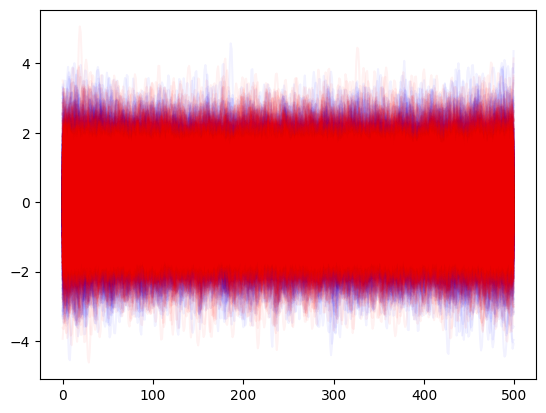
\includegraphics[width=\textwidth]{FordA}
        \caption*{FordA}
    \end{minipage}
    
    \vspace{0.4cm}
    
    \begin{minipage}[b]{0.32\textwidth}
        \centering
        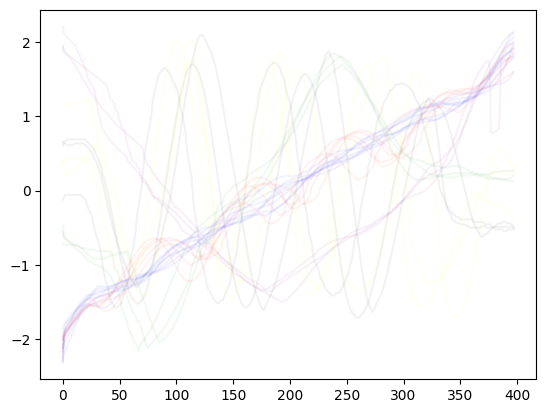
\includegraphics[width=\textwidth]{Symbols}
        \caption*{Symbols}
    \end{minipage}
    \hfill
    \begin{minipage}[b]{0.32\textwidth}
        \centering
        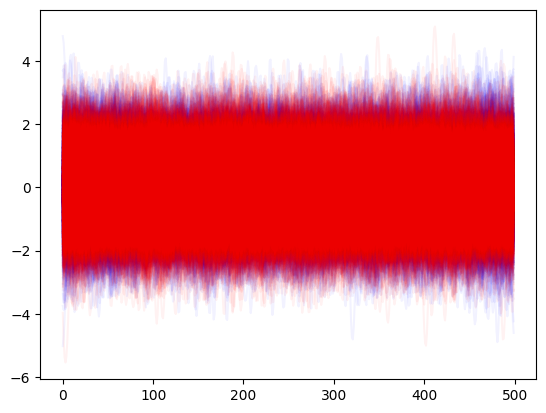
\includegraphics[width=\textwidth]{FordB}
        \caption*{FordB}
    \end{minipage}
    \hfill
    \begin{minipage}[b]{0.32\textwidth}
        \centering
        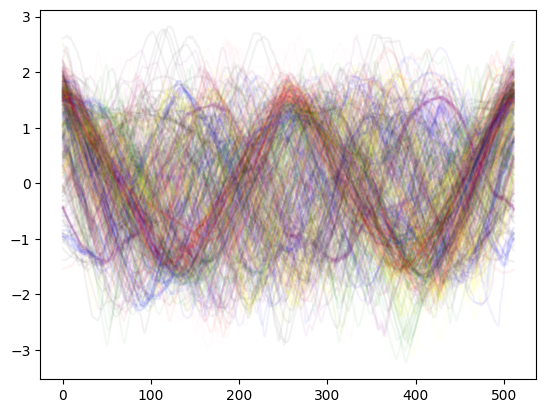
\includegraphics[width=\textwidth]{ShapesAll}
        \caption*{ShapesAll}
    \end{minipage}
    
    \vspace{0.4cm}
    
    \begin{minipage}[b]{0.32\textwidth}
        \centering
        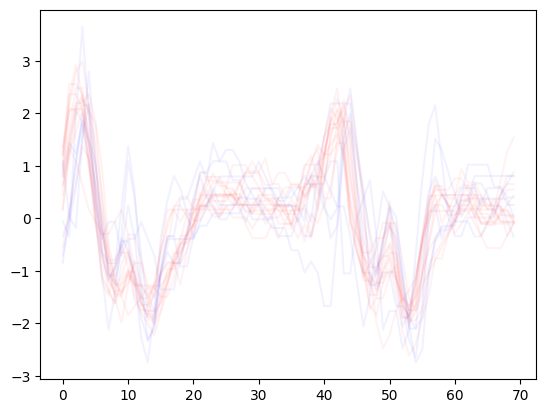
\includegraphics[width=\textwidth]{Sony1}
        \caption*{SonyAIBORobotSurface1}
    \end{minipage}
    \hfill
    \begin{minipage}[b]{0.32\textwidth}
        \centering
        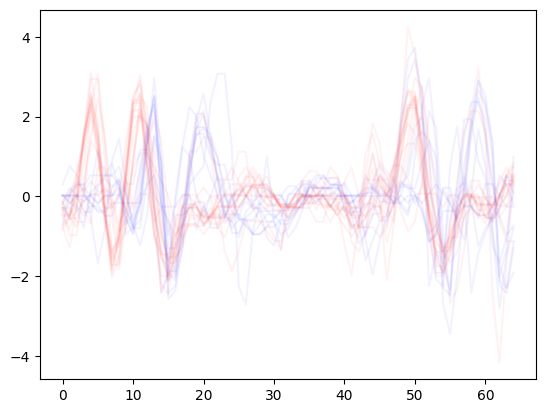
\includegraphics[width=\textwidth]{Sony2}
        \caption*{SonyAIBORobotSurface2}
    \end{minipage}
    \hfill
    \begin{minipage}[b]{0.32\textwidth}
        \centering
        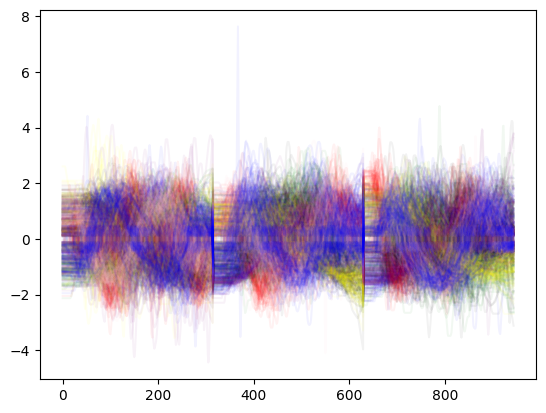
\includegraphics[width=\textwidth]{UWave}
        \caption*{UWaveGestureLibraryAll}
    \end{minipage}
    
    \vspace{0.4cm}
    
    \begin{minipage}[b]{0.32\textwidth}
        \centering
        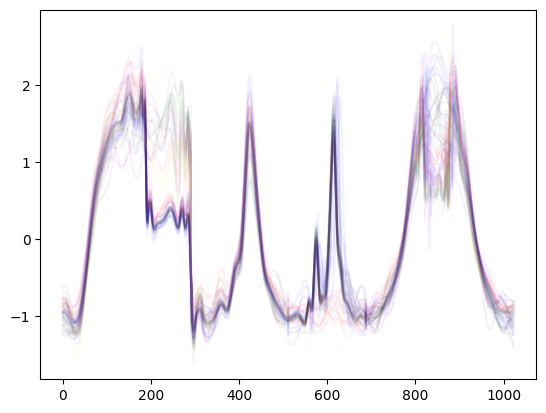
\includegraphics[width=\textwidth]{Mallat}
        \caption*{Mallat}
    \end{minipage}
    \caption{Our selected subset of the UCR Archive. All time series in the training set are plotted and color coded according to label.}
    \label{fig:datasets}
\end{figure}



\end{document}